% Generated through scripts/22_write_biometrics.py. Edit this template, not numerical output.
\documentclass[12pt,letterpaper]{article}
\usepackage[margin=1in]{geometry}
\usepackage[T1]{fontenc}
\usepackage{lmodern}
\usepackage{amsmath,amssymb,graphicx,booktabs,array,setspace}
\usepackage[authoryear,round]{natbib}
\usepackage[hidelinks]{hyperref}
\setstretch{1.85}
\setlength{\parindent}{1.5em}
\setlength{\parskip}{0pt}
\newcommand{\ind}{\mathbf{1}}
\begin{document}
\pagenumbering{roman}
\begin{titlepage}
\centering
\vspace*{1cm}
{\Large Design and outcome-model estimability in doubly robust survival analysis: a breast cancer reanalysis\par}
\vspace{1cm}
Wael Fahmy$^{*,\dagger}$, Elena Krikun$^{\dagger}$, and Abedalrhman Alkhateeb\par
Department of Computer Science, Lakehead University\par
955 Oliver Road, Thunder Bay, Ontario P7B 5E1, Canada\par
\vspace{1cm}
$^*$Corresponding author: \href{mailto:wfahmy@lakeheadu.ca}{wfahmy@lakeheadu.ca}\par
Contributing authors: \href{mailto:ekrikun@lakeheadu.ca}{ekrikun@lakeheadu.ca};
\href{mailto:aalkhate@lakeheadu.ca}{aalkhate@lakeheadu.ca}\par
$^\dagger$These authors contributed equally.\par
\vfill
Running title: Design and estimability in survival analysis\par
Article type: Biometric Practice\par
\end{titlepage}
\noindent\textbf{Summary.}
Doubly robust survival estimators require nuisance models that the available information can support.
We examine design and estimator dependence in TCGA breast cancer data.
Treatment indicators disagree for 337 of 1076 patients;
67.4\% have unobserved five-year binary outcomes; and receptor imputation expands
the triple-negative subgroup from 156 directly measured patients to 226.
We estimate adjusted restricted mean survival time (RMST) contrasts over 1095 days after a day-90 landmark.
Weighting-only estimates are 55 days (95\% bootstrap interval: -24, 133)
in triple-negative disease and 38 days (12, 72) in the whole cohort.
A Cox outcome-model benchmark yields 108 and 35 days, respectively,
demonstrating material model dependence in the smaller population.
A parameter-to-information ratio summarizes the burden on complete-outcome regressions within cross-fitting.
Its simulation-calibrated warning level is 0.31 (0.28--0.35) for the original regime;
additional simulations examine covariate-dependent censoring, delayed benefit and nonlinear misspecification.
The ratio does not certify estimator validity or replace weight diagnostics.
The contribution is a reproducible workflow that separates design, nuisance-model support and estimator stability
before interpreting observational survival contrasts.

\noindent\textbf{Key words:} Causal inference; Censoring; Doubly robust estimation; Landmark analysis; Nuisance estimation; Restricted mean survival time.
\clearpage
\pagenumbering{arabic}

\section{Introduction}
Public oncology cohorts invite treatment-effect questions that their clinical records were not necessarily
assembled to answer \citep{tcga}. Doubly robust estimation can reduce dependence on particular nuisance models
under appropriate assumptions \citep{chernozhukov,zhang}. It cannot resolve ambiguous treatment coding,
unobserved fixed-horizon outcomes, or a mismatch between treatment classification and follow-up origin.
Cross-fitting also does not guarantee satisfactory finite-sample performance when the outcome regression
has little information.

These problems are concrete in TCGA-BRCA. Two treatment indicators disagree for 337 of
1076 patients. A censoring-blind five-year mortality indicator assigns survival to
725 patients whose status at that horizon is unknown. Imputing receptor status expands
triple-negative breast cancer (TNBC) from 156 directly measured patients to 226.
These choices affect both the analysis population and the scientific question before an estimator is selected.

We organize the reanalysis around a sequence: specify the comparison, audit its observed-data construction,
account for censoring, examine information for nuisance estimation, and assess disagreement across estimators.
A landmark and an RMST contrast make time zero and the analysis horizon explicit
\citep{dafni,hernantrial,conner}. Unadjusted Kaplan--Meier, an adjusted Cox outcome model,
weighting-only survival estimation, and augmented inverse probability weighting (AIPW) are compared on
the same time scale. Simulation evaluates bias, precision, coverage and sensitivity rather than prediction accuracy.

Our diagnostic contribution is a parameter-to-information ratio for the complete-outcome regression
inside the studied AIPW estimator. Unlike prediction-model sample-size criteria
\citep{peduzzi,riley,vansmeden}, its calibration target is adjustment-set sensitivity relative to
sampling variability. It is a warning indicator, not a universal sample-size rule or an estimator-selection
theorem. Study-specific tools such as REFINE2 address the broader need to evaluate methods under realistic
data structures \citep{refine}. We add independent stress scenarios to examine how far the original
calibration can be transported.

\section{Materials and Methods}
\subsection{Analysis workflow and data}
Figure~\ref{fig:workflow} summarizes the workflow from input records to interpretation.
We use archived Genomic Data Commons clinical and follow-up exports and an earlier derived
UCSC Xena overall-survival table. The supplied survival table is reconciled with clinical records;
the original Xena export and original high-dimensional omics matrices are not included.
The earlier molecular adjustment set is supplied as a derived input, not reselected in this study.
Web Appendices B and I describe provenance and the exclusion ledger.

Receptor records retain positive, negative, equivocal, conflicting and untested states.
TNBC requires all three receptors to be directly recorded as negative; cohort-defining receptors
are never imputed. Indeterminate receptors exclude patients from the corresponding subgroup,
but not automatically from the whole-cohort chemotherapy analysis.

Chemotherapy and its first recorded start are derived from structured treatment-type and initiation-date fields.
The field is interpretable for this comparison but has not been validated against an external record standard.
Patients who die or are censored before day 90 are excluded, as are chemotherapy recipients without
a usable initiation date. Exposure is fixed at day 90 and follow-up is reset to that date.
Later initiators remain in the non-initiator group. We report TNBC and the whole cohort without
designating either population primary. Hormone therapy is a different treatment question and is not estimated here.

\subsection{Target contrast and assumptions}
Let $L=1$ denote eligibility for the analysis at the day-90 landmark, including being alive,
under follow-up and having classifiable treatment status; TNBC additionally requires measured receptors.
Let $A$ indicate chemotherapy initiation by day 90 and $X$ denote the adjustment covariates.
Survival and censoring times from the landmark are $T$ and $C$; we observe
$\widetilde T=\min(T,C)$ and $\delta=\ind(T\le C)$.
The statistical target is
\begin{equation}
\Delta(\tau)=E_{X\mid L=1}\left[\int_0^\tau
\{S(t\mid A=1,X,L=1)-S(t\mid A=0,X,L=1)\}\,dt\right],
\label{eq:target}
\end{equation}
with $\tau=1095$ days primary and 1825 days secondary. It compares initiation status by the landmark,
not chemotherapy with a sustained no-chemotherapy strategy.
Identification requires treatment positivity, positive censoring survival through the horizon,
and $C\perp T\mid A,X,L=1$. Causal interpretation additionally requires consistency for a
sufficiently specified treatment history and conditional exchangeability \citep{hernanbook}.

Landmarking avoids crediting follow-up before classification to the treated group, but does not
randomize treatment. Treated patients are prevalent users \citep{ray}; early treatment may affect
reaching the landmark. Conditioning on eligibility can therefore induce selection.
Neither the number excluded nor a second landmark bounds this bias.
The analysis does not emulate a trial assigning treatment at diagnosis or among untreated patients at day 90.

\subsection{Adjustment and preprocessing}
The primary clinical adjustment set represents age, stage, T, N and M category, calendar era and contributing site.
Site can proxy case mix, treatment practice, care and follow-up; association with treatment and outcome alone
does not establish confounding \citep{vanderweele}. Grade is entirely missing and a tumor-size field
is unavailable; T category is a coarse proxy. The earlier multimodal set and its union with the clinical
set are sensitivity specifications. Prognostic feature selection does not establish a valid confounder set.

Clinical continuous and ordinal missing values use median replacement with missingness indicators;
stage and TNM categories have fixed ordinal coding, and small sites are pooled.
The supplied earlier feature matrix uses its archived preprocessing, with remaining nonfinite values replaced
as documented in Web Appendix A. Clinical encoding, imputation and the supplied feature set are held fixed
for the reported resampling analysis. For AIPW, propensity/outcome scaling is computed on the analysis
matrix, while fitted regression coefficients and censoring-model training use the training folds.
This is not a fully nested feature-learning or preprocessing pipeline.
The clinical-first and weighting-only-first orderings were chosen after estimates were available;
they were not prospectively registered. Both estimators and all adjustment sets are retained.

\subsection{Survival estimators and comparator design}
The primary estimator combines stabilized treatment weights with time-varying inverse censoring weights
in a Kaplan--Meier product limit \citep{robins,conner}. Write $e(X)=\Pr(A=1\mid X,L=1)$,
$G(t\mid A,X)=\Pr(C>t\mid A,X,L=1)$ and $w_i=\Pr(A=A_i\mid L=1)/\Pr(A=A_i\mid X_i,L=1)$.
At the observed event times $t_j$ in arm $a$,
\begin{equation}
\widehat S_a(t)=\prod_{t_j\le t}\left[
1-\frac{\sum_{i:A_i=a}w_i\ind(\widetilde T_i=t_j,\delta_i=1)/\widehat G(t_j^-\mid a,X_i)}
{\sum_{i:A_i=a}w_i\ind(\widetilde T_i\ge t_j)/\widehat G(t_j^-\mid a,X_i)}
\right].\label{eq:km}
\end{equation}
Integrating the two curves gives an RMST contrast. Propensity is ridge logistic;
censoring uses a ridge Cox model stratified by treatment with shared covariate coefficients.
Both are fitted on the full analysis sample for this estimator. An arm-only censoring curve cancels
within each risk-set ratio, whereas covariate-conditional censoring weights do not.
Weighting-only estimation is not doubly robust.

The sensitivity estimator is a five-fold cross-fitted AIPW estimator of a complete restricted outcome:
death observed by $\tau$, or follow-up reaching $\tau$. Outcome regressions are IPCW-weighted ridge
least squares fitted within each treatment arm. Before truncation, its equation is doubly robust
in propensity and outcome regression conditional on a correct censoring model.
It omits the additional censoring augmentation used in more general survival estimators
\citep{bai,zhang}; Web Appendix A supplies the equation and expectation identity.
Cross-fitting alone does not establish nuisance-rate conditions or eliminate regularization bias.

Two benchmarks address different aspects of model dependence. Unadjusted Kaplan--Meier RMST describes
the observed treatment groups without confounder control. The adjusted outcome benchmark fits
$h(t\mid A,X)=h_0(t)\exp(\theta A+\beta^\top X)$ \citep{cox}, with an unpenalized treatment
coefficient and ridge-penalized standardized covariates. Its predicted survival under each treatment is
standardized over the same analysis population and integrated to the same $\tau$.
Thus its comparison with the adjusted estimators is in RMST days, not between a hazard ratio and a mean difference.
This death-hazard model is distinct from the Cox censoring model used in weighting.

Propensity limits are 0.01/0.99 for weighted KM and 0.02/0.98 for AIPW; censoring survival is floored at 0.05.
AIPW caps positive combined inverse weights at the 99th percentile and clips outcome predictions and
the final contrast to feasible ranges. These devices can introduce bias. We vary each separately and jointly.
The ridge rule, clipping conventions, weighting diagnostics and exploratory proportional-hazards screens
are specified in Web Appendices A, C, D and G.

\subsection{Information diagnostic and simulation assessment}
For $p$ outcome-model parameters, including the intercept after constant columns are removed,
$K$ folds and $c_{\min}$ complete restricted outcomes in the smaller treatment arm, define
\begin{equation}
\rho=\frac{p}{c_{\min}(1-1/K)}.\label{eq:rho}
\end{equation}
The denominator is an expected training-fold count; actual partitions differ.
The diagnostic precedes effect-model fitting but is not outcome-blind because completeness depends
on follow-up and event status. It applies to this complete-outcome regression, not automatically to
survival learners that use censored observations differently. We report effective degrees of freedom
from the actual Cox-weighted outcome fits beside nominal dimension.

The original calibration has 32 cells crossing sample sizes 150, 300, 600 and 1000,
covariate dimensions 10, 25, 50 and 75, and two event-rate settings, with 60 replicates per cell.
Covariates are Gaussian, treatment is logistic, survival exponential and censoring covariate-independent.
The first three covariates contain the treatment-assignment predictors, and all three nested adjustment
sets retain them. The calibration target is the mean within-replicate range across adjustment sets divided
by the full-set estimator's sampling standard deviation. A log-linear fit against $\rho$ defines the crossing
at 0.50, a chosen warning convention. Cell-bootstrap intervals, other crossing levels and penalty sensitivities
are reported in Web Appendix F. This is not a calibration to acceptable bias or coverage.

We add six independent stress cells: sample sizes 136 and 988 with 24 and 27 covariates, respectively,
crossed with covariate-dependent censoring under proportional hazards, delayed treatment benefit,
and heavy-tailed covariates with nonlinear propensity, survival and censoring mechanisms.
Each cell uses 200 replicates and 199 inner patient bootstraps.
Baseline hazards are calibrated to expected event counts near 16 or 72.
Analytic conditional RMST provides the replicate's covariate-standardized truth.
We compare all four estimators using bias, root mean squared error (RMSE), interval coverage,
standard-error calibration, failures and adjustment-set sensitivity. Monte Carlo uncertainty is reported,
including Wilson intervals for coverage. These scenarios test behavior outside the original grid;
they do not supply external clinical validation. Web Appendix G gives all mechanisms and results.

\subsection{Uncertainty and sensitivity analyses}
Clinical contrast intervals are patient-level percentile bootstrap intervals from 2000 replicates,
refitting the estimators on each resampled fixed covariate matrix. New KM/Cox benchmarks use the same
bootstrap draws as each other; existing estimators retain their documented seeds.
No synthetic oversampling is used. The original operating-point simulation uses 500 replicates per scenario
with 500 inner bootstraps, and is retained separately from the new stress study.
Additional checks vary adjustment sets, censoring models, stabilizers, landmark and horizon, and repeat
AIPW over 50 partitions and the core analysis over six seeds.
The correction ladder changes one design component at a time on a common RMST scale; its rungs need
not have an unchanged target. Exploratory heterogeneity is retained descriptively in Web Appendix H;
its earlier fixed-score intervals do not support confirmatory inference.

\section{Results}
\subsection{Cohort construction and observed follow-up}
Of 1076 patients, 57 do not reach the landmark,
29 have chemotherapy without a usable start date, and 2
have implausible prediagnosis starts, leaving 988.
Of these, 400 initiated chemotherapy by day 90 and 145 initiate later.
TNBC contains 136 patients, with 90 initiators and 46 non-initiators.
Deaths within the primary horizon number 16 and 72 in TNBC and the whole cohort.
Only 6 HER2-positive patients initiated targeted therapy by the landmark; no targeted-therapy contrast is estimated.

Median reverse-Kaplan--Meier follow-up in the original cohort is 974 days.
At five years, 201 patients are observed alive without a subsequent recorded death,
100 died by that horizon, 50 die later and therefore survived the horizon,
and 725 are censored earlier. Only the last group has unknown five-year status.
Coding them as survivors is unjustified even under independent censoring.
Web Appendix B presents the cohort ledger and follow-up figures.

\subsection{Same-horizon estimator comparison}
Table~\ref{tab:comparison} gives all four estimators under the clinical specification.
In TNBC, weighting-only estimation gives 55.0 days (95\% interval: -24.4, 132.5),
and AIPW gives 19.5 (-118.5, 179.7). The standardized Cox estimate is
108.3 (30.5, 167.6), compared with unadjusted KM 54.6 (-29.1, 144.7).
The Cox interval excludes zero while the weighted-KM and AIPW intervals span zero.
This disagreement shows model dependence on 16 deaths, not independent confirmation of benefit.

In the whole cohort, weighted KM gives 37.8 (12.1, 71.6),
Cox 35.4 (17.9, 55.1), and AIPW -8.3 (-32.6, 84.7).
The Cox and weighted-KM point estimates are close, while AIPW changes sign.
The unadjusted estimate is 41.5 (18.6, 64.7).
Each adjusted method relies on different modeling assumptions; agreement does not prove absence of confounding.

Across adjustment sets, TNBC weighted-KM estimates range from 28.6 to 55.0 days,
and AIPW from -5.4 to 42.0.
Changing covariate content changes nuisance fits and confounding control, so the difference cannot be
attributed to parameter count alone. At the secondary TNBC horizon, weighted KM gives 256 (32, 516) days
and AIPW 384 (107, 670) days; both intervals exclude zero, but tail support is limited.
The day-180 landmark gives whole-cohort AIPW 26.5 rather than -8.3 days;
both intervals include zero. Web Tables 2 and 6 retain the complete results.

\subsection{Information, balance and censoring support}
TNBC has 20/44 complete outcomes in controls/initiators,
25 nominal outcome-model parameters and $\rho=1.56$.
The whole cohort has 264/189 complete outcomes,
28 parameters and $\rho=0.19$.
In the smaller complete-outcome arm, actual training-fit effective degrees of freedom range
6.8--7.5 in TNBC and 17.1--18.4 in the whole cohort.
These are computed from the fitted cross-fold Cox-weighted regressions, not from an arm-only reference fit.

Under the primary KM treatment weights, mean absolute standardized differences change from
0.173 to 0.113 in TNBC and from 0.173 to 0.051
in the whole cohort; the corresponding maximum post-weighting differences are 0.379 and 0.196.
AIPW's capped complete-outcome residual-weight effective sample sizes are 31/7 and 77/86
for treated/control patients. These are estimator-specific weight summaries, not a universal sample size
or a direct variance formula for weighted KM. Full balance and support diagnostics accompany the code.

Across 15 sites with at least 20 patients, median follow-up ranges from 293 to 5086 days.
The censoring floor binds on 0/4 complete cases in the two weighted-KM fits
and 2/7 in cross-fitted AIPW.
Exploratory Schoenfeld screens of Efron-tie reference refits identify 1
covariate--process combinations after within-model Holm adjustment; year\_dx in the whole cohort censoring model (adjusted $p=0.0023$).
Penalization and few deaths limit these screens, and nonsignificance cannot establish proportional hazards
or independent censoring. Web Table 11 reports every tested term.

The revised five-device stabilizer analysis moves AIPW by up to 80.7 days;
weighted-KM shifts reach 10.2 days (Web Table 5).
Across 50 partitions, TNBC AIPW ranges from -134 to 81 days and whole-cohort AIPW from -19 to 29 days.
The original six-seed repeat gives weighted-KM interval excludes zero; AIPW interval spans zero.
Thus computational reproducibility under one seed does not imply partition stability.

\subsection{Calibration and independent stress assessment}
In the original grid, sensitivity is approximately $0.782+0.241\log\rho$
with $R^2=0.900$. The 0.50 crossing is 0.31 (cell-bootstrap interval 0.28--0.35).
Changing the crossing to 0.25 or 1.00 yields 0.11 or 2.47;
penalty multipliers 0.3 and 3 yield 0.22 or 1.32.
Figure~\ref{fig:calibration} juxtaposes the original calibration with the independent stress cells.
The maximum original-grid weighted-KM sensitivity ratio is 0.47, and the median AIPW/KM
movement ratio is 2.2. These are results for the tested implementations, not a general ranking.

Under proportional hazards with covariate-dependent censoring, coverage across adjusted methods and the two sample sizes ranges from 91.5 to 97.5\%, with absolute bias up to 14.0 days.

Under delayed benefit, coverage across adjusted methods and the two sample sizes ranges from 63.5 to 97.0\%, with absolute bias up to 19.2 days.

Under nonlinear heavy-tailed misspecification, coverage across adjusted methods and the two sample sizes ranges from 89.5 to 98.5\%, with absolute bias up to 5.7 days.

The lowest adjusted-method coverage occurs for Cox RMST at $n=988$ in the delayed benefit scenario: 63.5\% (95\% Monte Carlo interval 56.6--69.9\%).

There are 1 failed estimator--replicate evaluations across the stress study; coverage is conditional on successful evaluations, with failures reported separately.

Web Table 10 reports all four methods, including the confounded unadjusted benchmark, with RMSE, bias Monte Carlo errors and coverage uncertainty. The additional sensitivity points in Figure~\ref{fig:calibration} assess transport of the warning relationship; they do not recalibrate its crossing.

The original validation simulation gave coverage 92.2--95.8\% with absolute bias up to
12.5 days. Its distributions and covariate dimensions approximate aspects of the application;
they do not reproduce all site, missingness or treatment-selection processes.
Neither simulation study establishes the coverage of the clinical intervals.

\subsection{Design correction ladder}
Table~\ref{tab:ladder} retains every distinct RMST rung: 26.5, 40.1, 42.2, 54.6, 55.0 days.
The full progression is 28.6 days, compared with 35.5 days between weighted KM
and AIPW in the final TNBC clinical specification. The cohort contracts from 226 to 136.
The original censoring-blind binary risk differences are -7.6, -10.3, -9.1 percentage points;
they are an audit of the earlier endpoint and are not differenced against RMST.
Successive rungs change treatment classification, eligibility or time zero, so the progression is not an additive
decomposition of bias for one fixed estimand. Its magnitude is of similar order to estimator choice.

\section{Discussion}
The reanalysis separates three questions: whether the design defines a coherent comparison,
whether the outcome nuisance model has adequate information, and whether treatment and censoring weights
have support. The added Cox benchmark demonstrates why a conventional survival model is useful as a
comparator but cannot adjudicate the observational answer. Its TNBC interval excludes zero while the
other adjusted estimators disagree. In the whole cohort, weighted KM and Cox agree more closely,
yet the cross-fitted AIPW estimate is sensitive to weights and partitions.

The ratio $\rho$ describes one information burden. A high ratio should prompt simpler specifications,
fold-level checks or study-specific simulation; it neither proves invalidity nor selects weighted KM.
A low ratio cannot certify overlap, censoring support or stable weights. Its warning level depends on
the chosen crossing, penalties and data-generating regime. The independent stress study probes those limits
using known RMST truth, but a small collection of scenarios does not establish a universal boundary.
Effective complexity, stronger censoring diagnostics and other outcome learners require further calibration.

Clinical interpretation remains limited by prevalent treatment use, treatment-dependent landmark eligibility
and substantial scope for confounding by indication. Performance status, comorbidity, preference, grade and
size are incompletely measured or absent. Receptor records cannot resolve assay modality or clinically
adjudicate conflicts, and treatment records lack external validation. Some sites offer little follow-up at
the chosen horizon; truncation trades instability for potential bias. Covariate preprocessing and model order
were not prospectively fixed, and the reported bootstrap conditions on the constructed feature matrix.
The two populations overlap and the whole cohort pools distinct treatment indications.

This is a treatment-contrast estimation study. It does not develop a disease classifier, clustering procedure
or new molecular signature. Bias, coverage, RMSE and support therefore assess its statistical question;
classification accuracy or clustering indices would assess a different target. Functional enrichment can
interpret a selected gene set, but does not validate a treatment contrast. Independent clinical validation
would require dated treatment initiation, appropriately timed covariates, measured receptors and adequate
follow-up. Public treatment indicators alone are insufficient for reproducing the landmark design.

The published feature-selection framework \citep{krikun} supplies context for the earlier adjustment set;
we do not reassess its reported performance. Related manuscripts address treatment sequencing/initiation
and cross-cohort prognostic evaluation. Their current titles, submission statuses and overlap are disclosed
in Web Appendix J and the cover letter. This paper's conclusions concern the chemotherapy landmark
reanalysis and the behavior of an information diagnostic. They do not establish individual treatment benefit
or resolve chemotherapy effectiveness. The practical recommendation is to specify the target and analysis
ordering before inspecting contrasts, assess information and weight support, and report estimator disagreement.

\section*{Acknowledgments}
The results use data generated by the TCGA Research Network. This work received no specific grant
from public, commercial or not-for-profit funding agencies. The authors declare no conflicts of interest.

Author contributions: W.F. specified and implemented the reanalysis, estimators, diagnostic and
reproducibility pipeline and drafted the manuscript. E.K. designed and conducted the original study,
assembled the multi-omics cohort and revised the manuscript. A.A. supervised the work and provided
scientific framing. W.F. and E.K. contributed equally.

Generative AI tools (ChatGPT, OpenAI; Claude, Anthropic) assisted with code development and documentation,
manuscript drafting and revision, reference checking and document preparation. Patient-level source data
were not generated or altered by these tools. Numerical results were computed by the supplied analysis code.
The authors are responsible for verifying AI-assisted content and the final submission.

\section*{Data availability}
Public TCGA-BRCA records are distributed through the NCI Genomic Data Commons
(\href{https://portal.gdc.cancer.gov/projects/TCGA-BRCA}{TCGA-BRCA project portal})
and \href{https://xenabrowser.net}{UCSC Xena}.
The accompanying code-and-data supplement includes the archived clinical and derived analysis inputs,
input digests, exclusion ledger, analysis and simulation code, generated results and execution instructions.
Reproduction starts from these supplied inputs; it does not reconstruct the earlier omics feature-selection
pipeline from raw assay matrices. Only public, de-identified data are analyzed and no new participant contact occurs.


\begin{thebibliography}{99}
\bibitem[Bai et al.(2013)]{bai} Bai, X., Tsiatis, A. A., and O'Brien, S. M. (2013).
Doubly-robust estimators of treatment-specific survival distributions in observational studies with stratified sampling.
\textit{Biometrics} \textbf{69}, 830--839.
\bibitem[Cancer Genome Atlas Network(2012)]{tcga} Cancer Genome Atlas Network (2012).
Comprehensive molecular portraits of human breast tumours. \textit{Nature} \textbf{490}, 61--70.
\bibitem[Chernozhukov et al.(2018)]{chernozhukov} Chernozhukov, V., Chetverikov, D., Demirer, M.,
Duflo, E., Hansen, C., Newey, W., et al. (2018). Double/debiased machine learning for treatment
and structural parameters. \textit{The Econometrics Journal} \textbf{21}, C1--C68.
\bibitem[Conner et al.(2019)]{conner} Conner, S. C., Sullivan, L. M., Benjamin, E. J., LaValley, M. P.,
Galea, S., and Trinquart, L. (2019). Adjusted restricted mean survival times in observational studies.
\textit{Statistics in Medicine} \textbf{38}, 3832--3860.
\bibitem[Cox(1972)]{cox} Cox, D. R. (1972). Regression models and life-tables.
\textit{Journal of the Royal Statistical Society, Series B} \textbf{34}, 187--220.
\bibitem[Dafni(2011)]{dafni} Dafni, U. (2011). Landmark analysis at the 25-year landmark point.
\textit{Circulation: Cardiovascular Quality and Outcomes} \textbf{4}, 363--371.
\bibitem[Hern\'an and Robins(2020)]{hernanbook} Hern\'an, M. A. and Robins, J. M. (2020).
\textit{Causal Inference: What If}. Chapman and Hall/CRC, Boca Raton.
\bibitem[Hern\'an et al.(2016)]{hernantrial} Hern\'an, M. A., Sauer, B. C., Hern\'andez-D\'iaz, S.,
Platt, R., and Shrier, I. (2016). Specifying a target trial prevents immortal time bias and
other self-inflicted injuries in observational analyses. \textit{Journal of Clinical Epidemiology} \textbf{79}, 70--75.
\bibitem[Krikun and Alkhateeb(2026)]{krikun} Krikun, E. and Alkhateeb, A. (2026).
A Markov Blanket-based framework for dependency-aware feature selection in multimodal breast cancer data.
\textit{Network Modeling Analysis in Health Informatics and Bioinformatics} \textbf{15}, 158.
\bibitem[Meng and Huang(2026)]{refine} Meng, X. and Huang, J. Y. (2026).
REFINE2: a simplified simulation tool to help epidemiologists evaluate the suitability and sensitivity
of effect estimation within user-specified data. \textit{American Journal of Epidemiology} \textbf{195}, 533--542.
\bibitem[Peduzzi et al.(1996)]{peduzzi} Peduzzi, P., Concato, J., Kemper, E., Holford, T. R.,
and Feinstein, A. R. (1996). A simulation study of the number of events per variable in logistic regression
analysis. \textit{Journal of Clinical Epidemiology} \textbf{49}, 1373--1379.
\bibitem[Ray(2003)]{ray} Ray, W. A. (2003). Evaluating medication effects outside of clinical trials:
new-user designs. \textit{American Journal of Epidemiology} \textbf{158}, 915--920.
\bibitem[Riley et al.(2019)]{riley} Riley, R. D., Snell, K. I. E., Ensor, J., Burke, D. L.,
Harrell, F. E., Jr., Moons, K. G. M., et al. (2019). Minimum sample size for developing a multivariable
prediction model: Part II---binary and time-to-event outcomes. \textit{Statistics in Medicine} \textbf{38}, 1276--1296.
\bibitem[Robins and Finkelstein(2000)]{robins} Robins, J. M. and Finkelstein, D. M. (2000).
Correcting for noncompliance and dependent censoring in an AIDS clinical trial with inverse probability
of censoring weighted (IPCW) log-rank tests. \textit{Biometrics} \textbf{56}, 779--788.
\bibitem[van Smeden et al.(2016)]{vansmeden} van Smeden, M., de Groot, J. A. H., Moons, K. G. M.,
Collins, G. S., Altman, D. G., Eijkemans, M. J. C., et al. (2016).
No rationale for 1 variable per 10 events criterion for binary logistic regression analysis.
\textit{BMC Medical Research Methodology} \textbf{16}, 163.
\bibitem[VanderWeele(2019)]{vanderweele} VanderWeele, T. J. (2019). Principles of confounder selection.
\textit{European Journal of Epidemiology} \textbf{34}, 211--219.
\bibitem[Zhang and Schaubel(2012)]{zhang} Zhang, M. and Schaubel, D. E. (2012).
Double-robust semiparametric estimator for differences in restricted mean lifetimes in observational studies.
\textit{Biometrics} \textbf{68}, 999--1009.
\end{thebibliography}


\section*{Supplementary Material}
Web Appendices A--J, Web Tables 1--12, Web Figures 1--4, and the code-and-data supplement referenced in
Sections 2--4 accompany this paper. They provide estimator equations, preprocessing and audit provenance,
full numerical comparisons, diagnostic and sensitivity results, simulation designs and reproducibility instructions.

\clearpage
\begin{table}[p]
\setstretch{1.85}
\centering
\caption{RMST contrasts over 1095 days after the day-90 landmark. Intervals are 95\% patient-bootstrap
percentile intervals. The unadjusted benchmark compares observed groups; the adjusted methods target
the standardized contrast under their respective assumptions. Cox denotes an outcome model.}
\label{tab:comparison}
\setlength{\tabcolsep}{3pt}
\begin{tabular}{p{1.05in}p{1.45in}p{3.0in}}
\toprule Population & Estimator & Difference, days (95\% interval)\\\midrule
TNBC & Unadjusted KM & 54.6 (-29.1, 144.7) \\
TNBC & Weighted KM & 55.0 (-24.4, 132.5) \\
TNBC & AIPW & 19.5 (-118.5, 179.7) \\
TNBC & Cox RMST & 108.3 (30.5, 167.6) \\
Whole cohort & Unadjusted KM & 41.5 (18.6, 64.7) \\
Whole cohort & Weighted KM & 37.8 (12.1, 71.6) \\
Whole cohort & AIPW & -8.3 (-32.6, 84.7) \\
Whole cohort & Cox RMST & 35.4 (17.9, 55.1) \\
\bottomrule
\end{tabular}
\end{table}
\clearpage
\begin{table}[p]
\setstretch{1.85}
\centering
\caption{TNBC design correction ladder on a common 1095-day RMST scale.
Rungs 0--3 are unadjusted and rung 4 uses clinical weighted KM.
Event counts use each rung's time origin. Changing the binary endpoint to RMST is a change of target,
not an additional numerical rung. Each interval belongs to its own specification.}
\label{tab:ladder}
\setlength{\tabcolsep}{3pt}
\begin{tabular}{rp{2.1in}rrp{1.7in}}
\toprule Rung & Specification & $n$ & Deaths & RMST (95\% interval)\\\midrule
0 & Original coding and imputed TNBC & 226 & 25 & 26.5 (-28.6, 84.8) \\
1 & Structured chemotherapy field & 226 & 25 & 40.1 (-21.0, 105.9) \\
2 & Measured receptors only & 156 & 15 & 42.2 (-56.5, 164.8) \\
3 & Day-90 landmark & 136 & 16 & 54.6 (-35.6, 154.5) \\
4 & Clinical adjustment & 136 & 16 & 55.0 (-24.4, 132.5) \\
\bottomrule
\end{tabular}
\end{table}
\clearpage
\begin{figure}[p]
\setstretch{1.85}
\centering
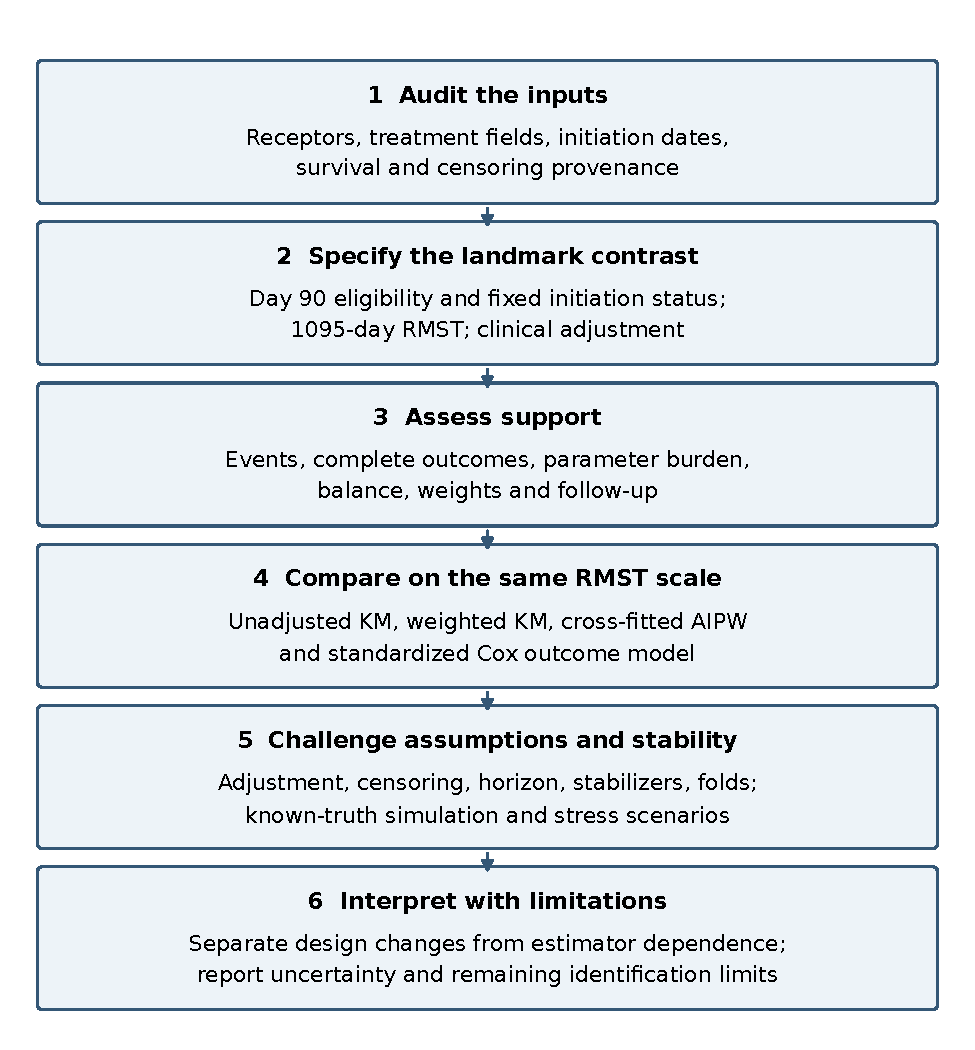
\includegraphics[width=\textwidth,height=0.70\textheight,keepaspectratio]{figures/fig7_workflow.pdf}
\caption{Analysis workflow, introduced at the beginning of Materials and Methods.
The information ratio, balance and follow-up support inform interpretation; they do not automatically
select an estimator or establish causal identification. The final step compares assumptions and sensitivity.}
\label{fig:workflow}
\end{figure}
\clearpage
\begin{figure}[p]
\setstretch{1.85}
\centering
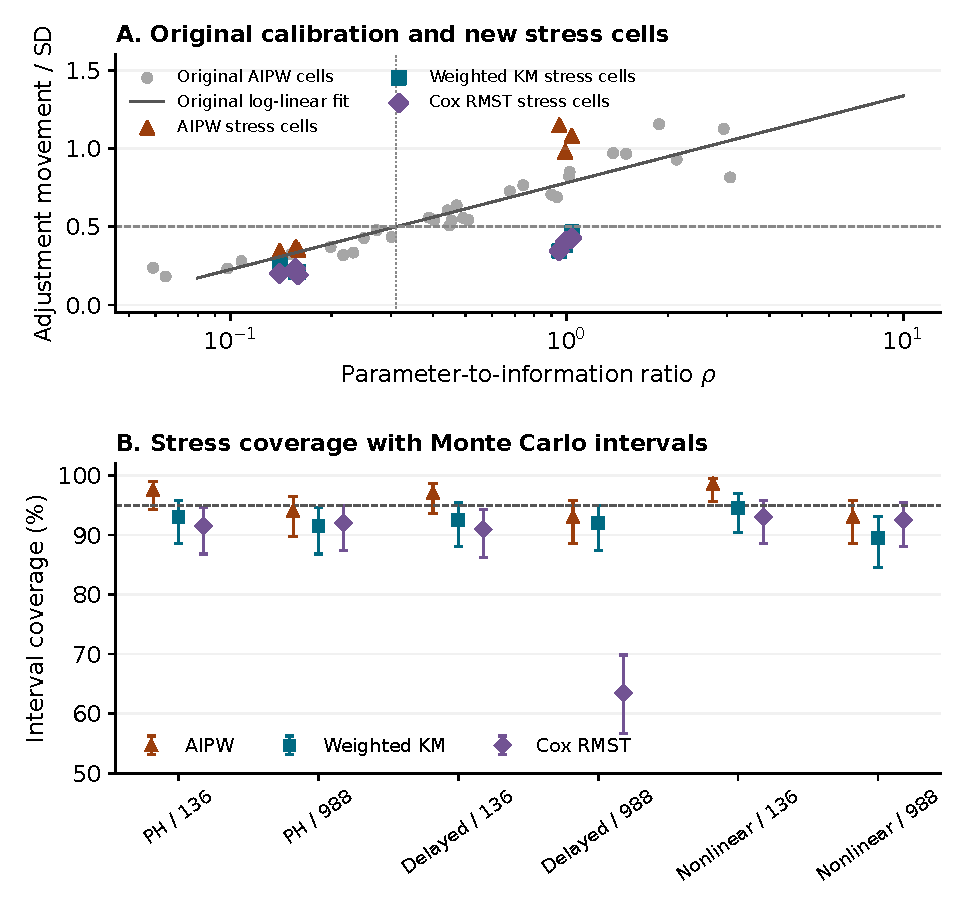
\includegraphics[width=\textwidth,height=0.70\textheight,keepaspectratio]{figures/fig8_calibration_stress.pdf}
\caption{Original calibration and independent stress assessment. The original log-linear AIPW fit
and its 0.50 crossing are shown with the original grid cells and new scenario means.
The lower panel gives coverage of nominal 95\% bootstrap intervals in the stress study; bars are 95\%
Wilson intervals for Monte Carlo uncertainty. These assess the simulated settings, not clinical coverage.
Weighted KM and AIPW denote the adjusted implementations; Cox uses standardized outcome-model survival.}
\label{fig:calibration}
\end{figure}
\end{document}
